\section{Алгоритмы решения задач с данными Коши. Примеры.}\label{sec:ch4/sec4}

%VYC0036
\subsection{
    Задачи сложного теплообмена
    с граничными условиями типа Коши на всей границе
}\label{subsec:ch4/sec4/subsec1}

Решим экстремальную задачу~\eqref{eq:2_2:eq1},~\eqref{eq:2_2:bc3},~\eqref{eq:2_2:cost}.
Для этого представим итерационный алгоритм решения задачи оптимального управления.
Пусть $\tilde J_\lambda(u)=J_\lambda(\theta(u), u)$, где $\theta(u)$ компонента решения
задачи~\eqref{eq:2_2:eq1},~\eqref{eq:2_2:bc2}, соответствующая управлению $u\in U$.

В соответствии с~\eqref{eq:2_2:as} градиент функционала $\tilde J_\lambda(u)$ равен
\[
    \tilde J'_\lambda (u) = \lambda u - p_2.
\]
Здесь $p_2$ -- соответствующая компонента сопряженного
состояния из системы~\eqref{eq:2_2:as}, где $\hat{\theta}\coloneqq\theta(u)$.

%\begin{algorithm}[H]
%    \caption{Алгоритм градиентного спуска}
%    \label{alg:algorithm}
%    \begin{algorithmic}[1]
%        \State Выбираем значение градиентного шага $\varepsilon$,
%        \State Выбираем количество итераций $N$,
%        \State Выбираем начальное приближение для управления $u_0 \in U$,
%        \For{$k \gets 0,1,2,\dots,N$}
%            \State Для данного $u_k$ рассчитываем состояние $y_k = \{\theta_k, \varphi_k\}$ --
%            решение задачи~\eqref{eq:2_2:eq1},~\eqref{eq:2_2:bc1}.
%            \State Рассчитываем значение функционала качества $J_\lambda(\theta_k, u_k)$.
%            \State Рассчитываем сопряженное состояние
%$p_k=\{p_{1k},p_{2k}\}$ из уравнений~\eqref{eq:2_2:oc1},
%            где $ \hat{\theta} \coloneqq \theta_k, \hat{u}=u_k$.
%            \State Пересчитываем управление $u_{k+1} = u_k - \varepsilon (\lambda u_k - p_2)$
%        \EndFor
%    \end{algorithmic}
%\end{algorithm}
\textbf{Алгоритм градиентного спуска}

1.\ Выбираем значение градиентного шага $\varepsilon$,

2.\ Выбираем количество итераций $N$,

3.\ Выбираем начальное приближение для управления $u_{0} \in U$,

4.\ для $k \leftarrow 0,1,2, \ldots, N$ выполнить:

\hspace{1cm} a.\ Для заданного $u_{k}$, вычислить состояние
$y_{k}=\left\{\theta_{k}, \varphi_{k}\right\}$, решение
задачи~\eqref{eq:2_2:eq1}--\eqref{eq:2_2:bc1}.

\hspace{1cm} b.\ Вычислить значение функционала качества
$J_{\lambda}\left(\theta_{k}, u_{k}\right)$.

\hspace{1cm} c.\ Из уравнений~\eqref{eq:2_2:oc1}, вычислить сопряженное
состояние $p_{k}=\left\{p_{1k}, p_{2k}\right\}$,
где $\widehat{\theta} \coloneqq \theta_{k}, \widehat{u} \coloneqq u_{k}$.

\hspace{1cm} d.\ Пересчитать управление
$u_{k+1}=u_{k}-\varepsilon\left(\lambda u_{k}-p_{2}\right)$.


Значение параметра $\varepsilon$ выбирается эмпирически таким образом, чтобы значение
$\varepsilon (\lambda u_k - p_2)$ являлось существенной поправкой для $u_{k+1}$.
Количество итераций $N$ выбирается достаточным для выполнения условия
$J_\lambda(\theta_k, u_k) - J_\lambda(\theta_{k+1}, u_{k+1}) < \delta$, где $\delta>0$
определяет точность расчетов.

Примеры, рассмотренные ниже, иллюстрируют работоспособность предложенного алгоритма при
малых, что важно, значениях параметра регуляризации $\lambda \leq 10^{-12}$.
В первом примере выполнены тестовые расчеты для куба.
Во втором примере приводится сравнение расчетов по
предложенному алгоритму с результатами работы~\cite{Chebotarev2019Problem}.

Для численного решения прямой задачи с заданным управлением использовался
метод Ньютона для линеаризации задачи и ее решения методом конечных элементов.
Решение сопряженной системы, которая является линейной при заданной температуре,
не вызывает трудностей.
Для численного моделирования использовался солвер FEniCS~\cite{fenics, dolfin}.

Исходный код экспериментов представлен в открытом доступе~\cite{mesenev-github}.

\textbf{Пример 1.}
Приведем примеры расчетов для куба $\Omega = {(x, y, z), 0 \leq x,y,z \leq l}$.
Будем считать, что $l=1~\text{см}$, $a = 0.006[\text{см}^2/\text{c}]$,
$b=0.025[\text{см}/\text{с}]$, $\kappa_a=1[\text{см}^{-1}]$, $\alpha = 0.(3)[\text{см}]$.
Указанные параметры соответствуют стеклу~\cite{Grenkin2016a}.
Параметр регуляризации $\lambda=10^{-12}$.

Пусть граничные данные $r$ и $u$ в~\eqref{eq:2_2:bc3} имеют вид:
\[
    r = 0.7, \quad
    u = \hat u = 0.5.
\]
Далее рассчитываем состояние $\theta$ и $\varphi$ как решение
задачи~\eqref{eq:2_2:eq1},~\eqref{eq:2_2:bc3} и в качестве $\theta_b$
выбираем граничное значение функции $\theta$ на $\Gamma$.
Значения нормальной производной $\partial_n\theta$ на $\Gamma$
должны соответствовать значениям $q_b=r/a-\theta_b$.
Применяя предложенный алгоритм с начальным приближением $u_0 = 0.1$,
находим приближенное решение $\{\theta_\lambda, \varphi_\lambda, u_\lambda\}$ задачи $CP$.
Для демонстрации того, что алгоритм находит приближенное решение задачи с данными
Коши для температуры, важно сравнить значения $\partial_n\theta_\lambda$ на $\Gamma$ с $q_b$.

На рисунке~\ref{fig:4_4:0}а представлен модуль относительного
отклонения $\partial_n\theta_\lambda$ от $q_b$ на грани куба в плоскости $z=l$,
где $\partial_n\theta_\lambda=\partial\theta_\lambda/\partial z$,
а также динамика функционала качества, определяющего норму
разности $\|\theta_\lambda -\theta_b\|^2_\Gamma$ на рисунке~\ref{fig:4_4:0}б.
На остальных гранях куба значения относительного
отклонения имеют тот же порядок малости.

\begin{figure}[h!t]
    \begin{minipage}[b][][b]{0.49\linewidth}
        \centering
        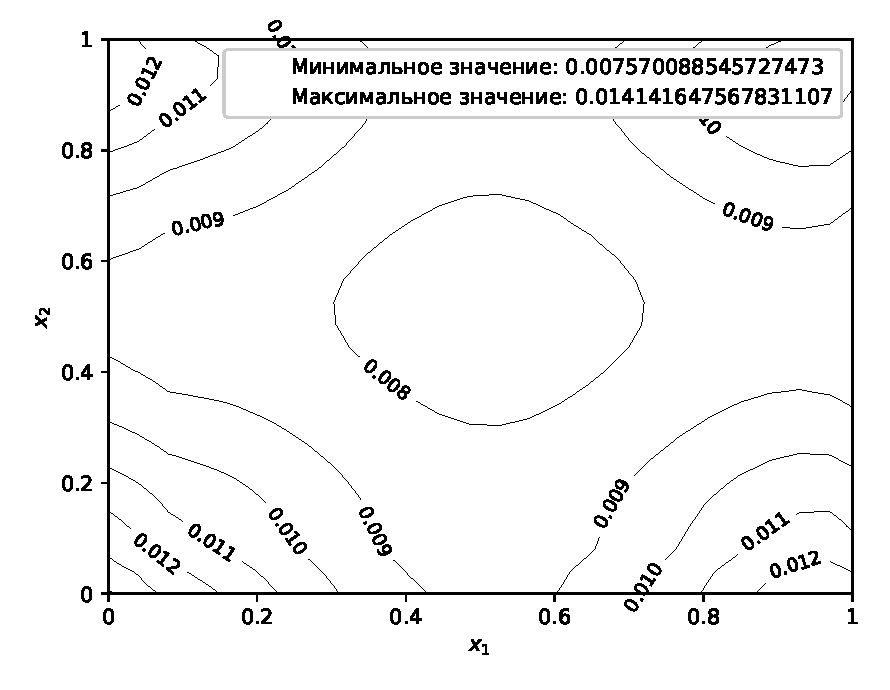
\includegraphics[width=1\linewidth]{jvm-2020/exp1/theta_n_diff_iso}
        \\ а) $|\partial_n\theta_\lambda-q_b|/|q_b|$
    \end{minipage}
    \hfill
    \begin{minipage}[b][][b]{0.49\linewidth}
        \centering
        \includegraphics[width=1\linewidth]{jvm-2020/exp1/quality}
        \\ б) Значение функционала качества
    \end{minipage}
    \caption{Результаты первого эксперимента}
    \label{fig:4_4:0}
\end{figure}

\textbf{Пример 2.}
Задача рассматривается в области $\Omega \times (-L,L)$,
где $\Omega = \{ x = (x_1,x_2) \colon 0 < x_{1,2} < d\}$
и при больших $L$ сводится к двумерной задаче с вычислительной областью $\Omega$.
Выбраны следующие значения параметров задачи:
$d = \mathrm{1(m)}$, $a = 0.92~10^{-4}~\mathrm{(m^2/s)}$, $b= 0.19~\mathrm{(m/s)}$,
$\alpha = 0.0333~\mathrm{(m)}$ и $\kappa_a = 1~\mathrm{(m^{-1})}$.
Параметры соответствуют воздуху при нормальном атмосферном давлении и температуре $400^\circ$C.

Функции $\theta_b$, $q_b$ в краевом условии~\eqref{eq:2_2:bc2} заданы следующим образом:
\[
    \theta_b = \widehat{\theta}|_{\Gamma}, \quad q_b = \partial_n \widehat{\theta}|_{\Gamma},
\]
где $\widehat{\theta} = (x_1-0.5)^2 - 0.5x_2+0.75$.


На рис.~\ref{fig:4_4:1}а представлено температурное поле, полученное
предложенным методом.
Величина $\|\partial_n\theta_\lambda-q_b\|_{L^2(\Gamma)}/\|q_b\|_{L^2(\Gamma)}$ равна $0.000567$.
Значение функционала качества, определяющего норму разности $\|\theta_\lambda -\theta_b\|^2_\Gamma$,
равно $~0.000255$ и стабилизируется после 10 итераций.
Динамика функционала качества представлена на рис.~\ref{fig:4_4:1}б.

\begin{figure}[h!t]
    \begin{minipage}[b][][b]{0.49\linewidth}
        \centering
        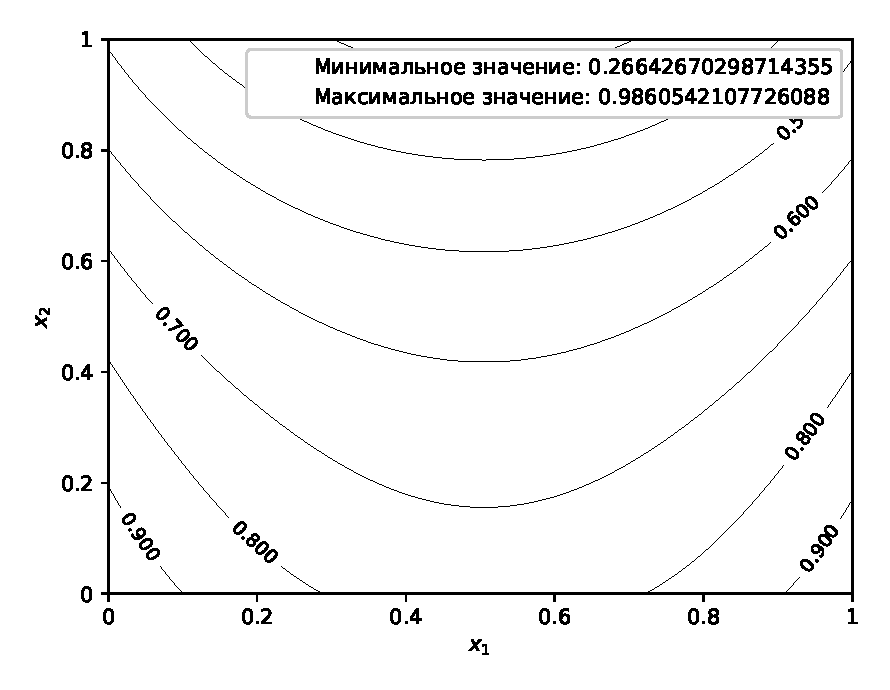
\includegraphics[width=1\linewidth]{jvm-2020/exp2/theta_auto}
        \\ а) Полученное решение $\theta$
    \end{minipage}
    \hfill
    \begin{minipage}[b][][b]{0.49\linewidth}
        \centering
        \includegraphics[width=1\linewidth]{jvm-2020/exp2/quality}
        \\ б) Изменение функционала качества
    \end{minipage}
    \caption{Результаты второго эксперимента}
    \label{fig:4_4:1}
\end{figure}

Представленные численные примеры иллюстрируют, что предложенный алгоритм успешно справляется
с нахождением численного решения задачи~\eqref{eq:2_2:eq1}--\eqref{eq:2_2:bc2}.


\textbf{Пример 3.}
Положим в условии~\eqref{eq:2_2:bc3}
$r=0.8 \cos (x)+0.1,\; u=\hat{u}=y$.
Далее рассчитываем состояние $\theta$ и $\varphi$ как решение
задачи~\eqref{eq:2_2:eq1}--\eqref{eq:2_2:bc2}
и в качестве $\theta_{b}$ выбираем граничные значения функции $\theta$ на Г.
Применяя предложенный алгоритм с начальным приближением $u_{0}=0.1$,
находим приближенное решение задачи $CP$.
Квадрат разницы тестового и найденного решения представлен на рисунке~\ref{fig:4_4:2}а,
динамика функционала качества представлена на рисунке~\ref{fig:4_4:2}б.

\begin{figure}[h!t]
    \begin{minipage}[b][][b]{0.49\linewidth}
        \centering
        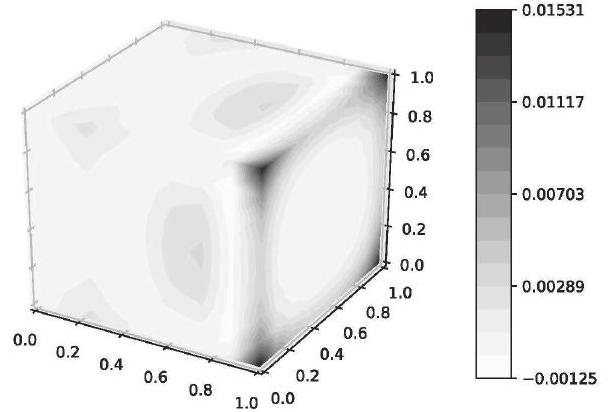
\includegraphics[width=1\linewidth]{jvm-2020/dvmg/1a}
        \\ а) $\left(\hat{u}-u_{100}\right)^{2}$
    \end{minipage}
    \hfill
    \begin{minipage}[b][][b]{0.49\linewidth}
        \centering
        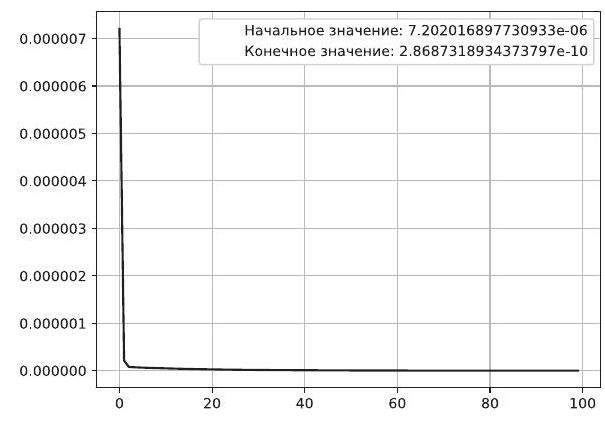
\includegraphics[width=1\linewidth]{jvm-2020/dvmg/1b}
        \\ б) Изменение функционала в зависимости от числа итераций
    \end{minipage}
    \caption{Результаты третьего эксперимента}
    \label{fig:4_4:2}
\end{figure}


\textbf{Пример 4.}
Зададим функции $\theta_{b}, q_{b}$ в краевом условии~\eqref{eq:2_2:bc2}
следующим образом:
\[
    \theta_{b}=0.1 z+0.3, \quad q_{b}=
    \begin{cases}
        0.11, & \text { если } z=1, \\
        0, & \text { если } 0<z<1, \\
        -0.15, & \text { если } z=0.
    \end{cases}
\]


В данном примере оптимальное управление $u$ в качестве тестового не задается.
На рисунках~\ref{fig:4_4:3}а,~\ref{fig:4_4:3}б представлен результат работы алгоритма.

\begin{figure}[h!t]
    \begin{minipage}[b][][b]{0.49\linewidth}
        \centering
        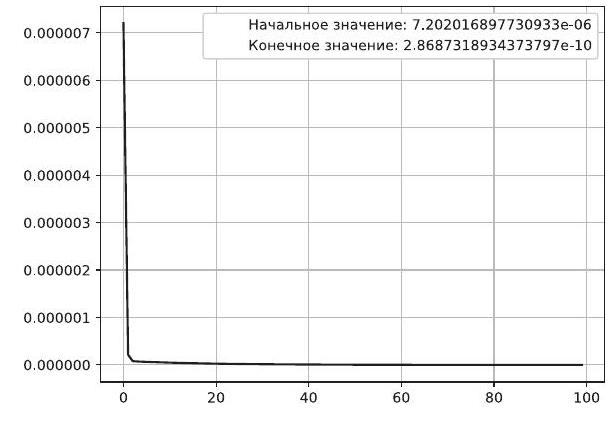
\includegraphics[width=0.9\linewidth]{jvm-2020/dvmg/3a}
        \\ а) Изменение функционала в зависимости от числа итераций
    \end{minipage}
    \hfill
    \begin{minipage}[b][][b]{0.49\linewidth}
        \centering
        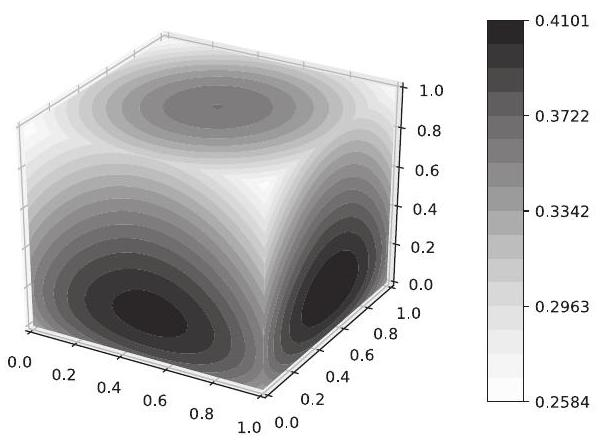
\includegraphics[width=1\linewidth]{jvm-2020/dvmg/2b}
        \\ б) Оптимальное управление
    \end{minipage}
    \caption{Результаты четвёртого эксперимента}
    \label{fig:4_4:3}
\end{figure}

Компоненты состояния, соответствующие найденному управлению, представлены на
рисунках~\ref{fig:4_4:4}а,~\ref{fig:4_4:4}б.


\begin{figure}[h!t]
    \begin{minipage}[b][][b]{0.49\linewidth}
        \centering
        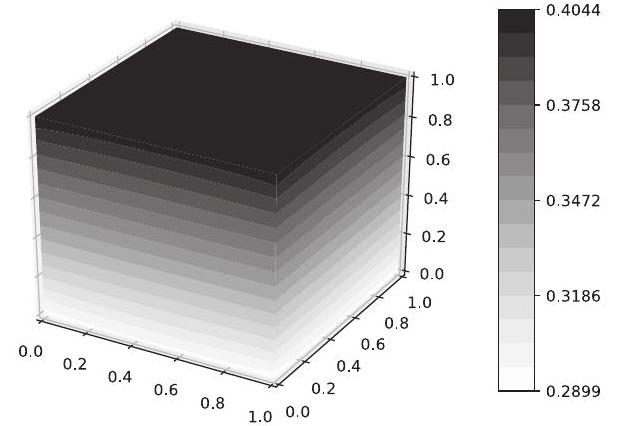
\includegraphics[width=1\linewidth]{jvm-2020/dvmg/3b}
        \\ а) Температура $\theta$
    \end{minipage}
    \hfill
    \begin{minipage}[b][][b]{0.49\linewidth}
        \centering
        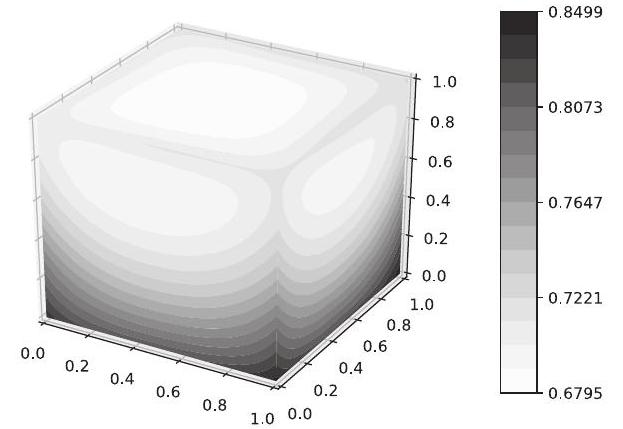
\includegraphics[width=1\linewidth]{jvm-2020/dvmg/2a}
        \\ б) Излучение $\varphi$
    \end{minipage}
    \caption{Результаты четвёртого эксперимента}
    \label{fig:4_4:4}
\end{figure}

\subsection{
    Задача сложного теплообмена с условиями
    Коши для температуры на части границы
}\label{subsec:ch4/sec4/subsec2}
%jvm-mesenev-chebotarev

Задача оптимального управления, сформулированная в разделе~\ref{subsec:ch2/sec4/state},
заключается в отыскании тройки $\{\theta_\lambda,\psi_\lambda,u_\lambda\}$ такой, что
\begin{gather*}
    J_\lambda(\theta, u) =
    \frac{1}{2} \int \limits_{\Gamma_1} (\theta - \theta_b)^2 d \Gamma
    + \frac{\lambda}{2}\int\limits_{\Gamma_2} u^2 d\Gamma \rightarrow \inf, \\
    - a \Delta \theta + g (\theta) = \frac{\kappa}{\alpha}\psi, \quad
    \Delta \psi = 0, \; x \in \Omega, \\
    a \partial_n \theta + s \theta = q_b + s \theta_b,
    \; \alpha \partial_n \psi + \gamma \psi = r
    \text{ на } \Gamma_1,\\
    a \partial_n \theta = q_b, \;
    \alpha \partial_n \psi = u \text{ на } \Gamma_2,
\end{gather*}
где $\lambda, s > 0$ -- регуляризирующие параметры.


Представим итерационный алгоритм решения задачи оптимального управления.
Пусть $\tilde J_\lambda(u)=J_\lambda(\theta(u), u)$,
где $\theta(u)$ компонента решения
задачи~\eqref{eq:2_4:eq1},~\eqref{eq:2_4:bc2}, соответствующая управлению $u\in U$.

В соответствии с~\eqref{eq:2_4:as} градиент функционала $\tilde J_\lambda(u)$ равен
\[ \tilde J'_\lambda (u) = \lambda u - p_2. \]
Здесь $p_2$ -- соответствующая компонента сопряженного состояния из системы ~\eqref{eq:2_4:as},
где $\hat{\theta}\coloneqq\theta(u)$.

%    \begin{algorithm}[H]
%        \caption{Алгоритм градиентного спуска}
%        \label{alg:algorithm}
%        \begin{algorithmic}[1]
%            \State Выбираем значение градиентного шага $\varepsilon$,
%            \State Выбираем количество итераций $N$,
%            \State Выбираем начальное приближение для управления $u_0 \in U$,
%            \For{$k \gets 0,1,2,\dots,N$}
%                \State Для данного $u_k$ рассчитываем состояние $y_k = \{\theta_k, \varphi_k\}$ --
%                решение задачи~\eqref{eq1},~\eqref{bc1}.
%                \State Рассчитываем значение целевого функционала $J_\lambda(\theta_k, u_k)$.
%                \State Рассчитываем сопряженное состояние
%$p_k=\{p_{1k},p_{2k}\}$ из уравнений ~\eqref{OC1},
%                где $ \hat{\theta} \coloneqq \theta_k, \hat{u}=u_k$.
%                \State Пересчитываем управление $u_{k+1} = u_k - \varepsilon (\lambda u_k - p_2)$
%            \EndFor
%        \end{algorithmic}
%    \end{algorithm}
Значение параметра $\varepsilon$ выбирается эмпирически таким образом, чтобы значение
$\varepsilon (\lambda u_k - p_2)$ являлось существенной поправкой для $u_{k+1}$.
Количество итераций $N$ выбирается достаточным для выполнения условия
$J_\lambda(\theta_k, u_k) - J_\lambda(\theta_{k+1}, u_{k+1}) < \delta$, где $\delta > 0$
определяет точность расчетов.

В первом примере выполнены тестовые расчеты для куба.
Во втором примере рассмотрен куб с внутренней полостью.
Для численного решения прямой задачи с заданным управлением использовался
метод Ньютона для линеаризации задачи и ее решения методом конечных элементов.
Решение сопряженной системы, которая является линейной
при заданной температуре, не вызывает трудностей.
Для численного моделирования использовался солвер FEniCS~\cite{fenics},\cite{dolfin}.
Исходный код экспериментов представлен в открытом доступе~\cite{mesenev-github}.

\textbf{Пример 1.}
Рассмотрим куб $\Omega = \{ (x, y, z), 0 \leq x,y,z \leq l \}$ с границей
$\Gamma \equiv \Gamma_1 \cup \Gamma_2$, где
\[
    \Gamma_1 = \{(x, y, z), 0 \leq x,y, \leq l, z \in 0, l\}, \;
    \Gamma_2 = \partial \Omega \setminus \Gamma_1.
\]
Будем считать, что
$l = 1~\text{см}$,
$a = 0.6[\text{см}^2/\text{c}]$,
$b = 0.025[\text{см}/\text{с}]$,
$\kappa_a = 1[\text{см}^{-1}]$,
$\alpha = 0.(3)[\text{см}]$.
Указанные параметры соответствуют стеклу~\cite{Grenkin2016a}.
Параметр регуляризации $\lambda=10^{-12}$.

Пусть граничные данные $q_b$ и $\theta_b$ в~\eqref{eq:2_4:bc1},~\eqref{eq:2_4:bc2} имеют вид:
\begin{gather*}
    q_b = 0.5, \quad
    \theta_b = 0.1 + z/2
\end{gather*}
на всей границе, а также начальное управление $u_0 = 0$.
Используя предложенный алгоритм, решим задачу оптимального управления.

\begin{figure}[h!t]
    \begin{minipage}[b][][b]{0.49\linewidth}
        \centering
        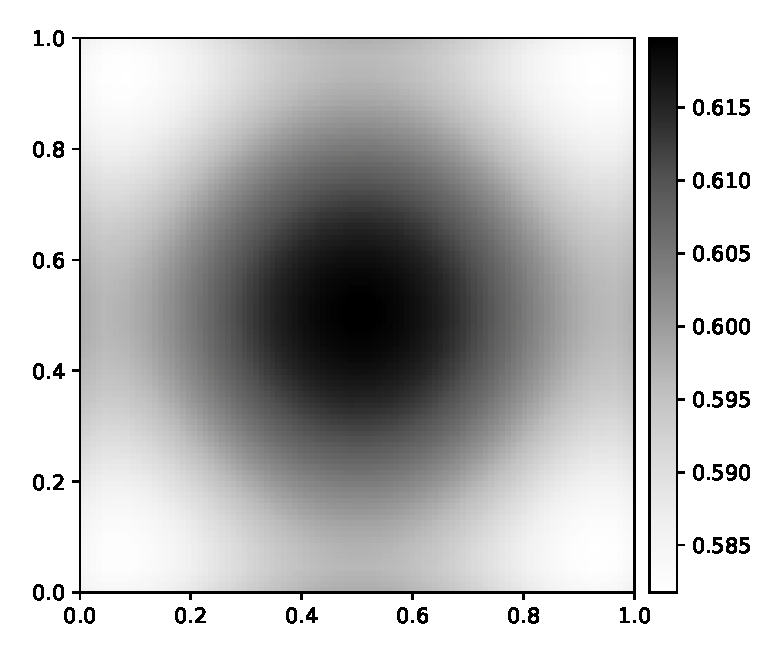
\includegraphics[width=1\linewidth]{jvm-2022/1_theta}
        \\ а) $\theta|_{z=1}$
    \end{minipage}
    \hfill
    \begin{minipage}[b][][b]{0.49\linewidth}
        \centering
        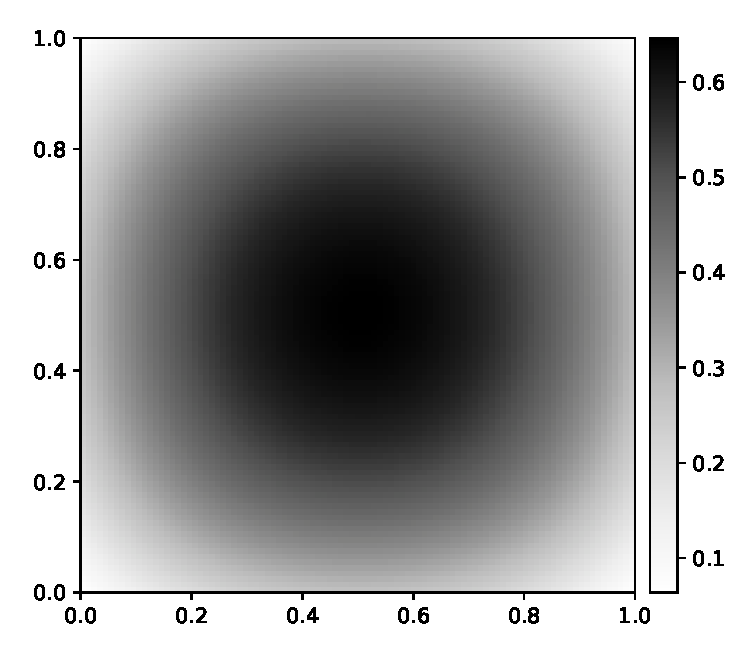
\includegraphics[width=1\linewidth]{jvm-2022/1_phi}
        \\ б) $\varphi|_{z=1}$
    \end{minipage}
    \caption{Результаты первого эксперимента}
    \label{fig:4_4:5}
\end{figure}

На рисунке~\ref{fig:4_4:5}а,~\ref{fig:4_4:5}б представлены
полученные решения $\theta$ и $\phi$.
Начальное значение функционала качества равно $0.025$ и
через сотню итераций становится равным $5\cdot 10^{-5}$.

\textbf{Пример 2.}
\begin{figure}[h!t]
    \begin{minipage}[b][][b]{0.49\linewidth}
        \centering
        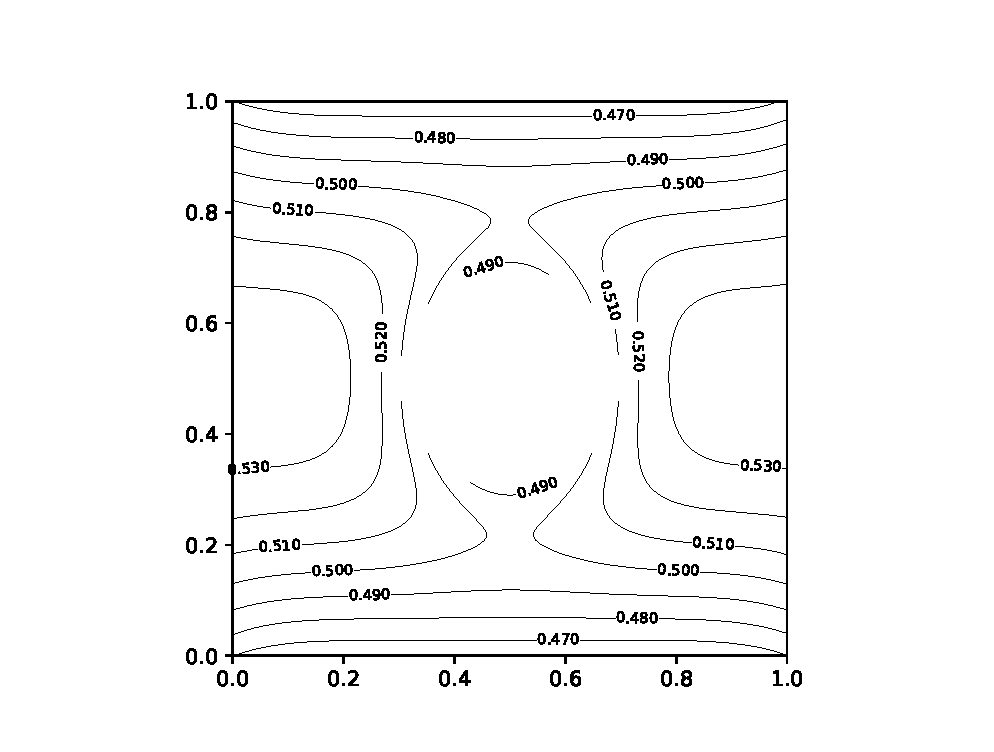
\includegraphics[width=1\linewidth]{jvm-2022/2_theta}
        \\ а) $\theta$
    \end{minipage}
    \hfill
    \begin{minipage}[b][][b]{0.49\linewidth}
        \centering
        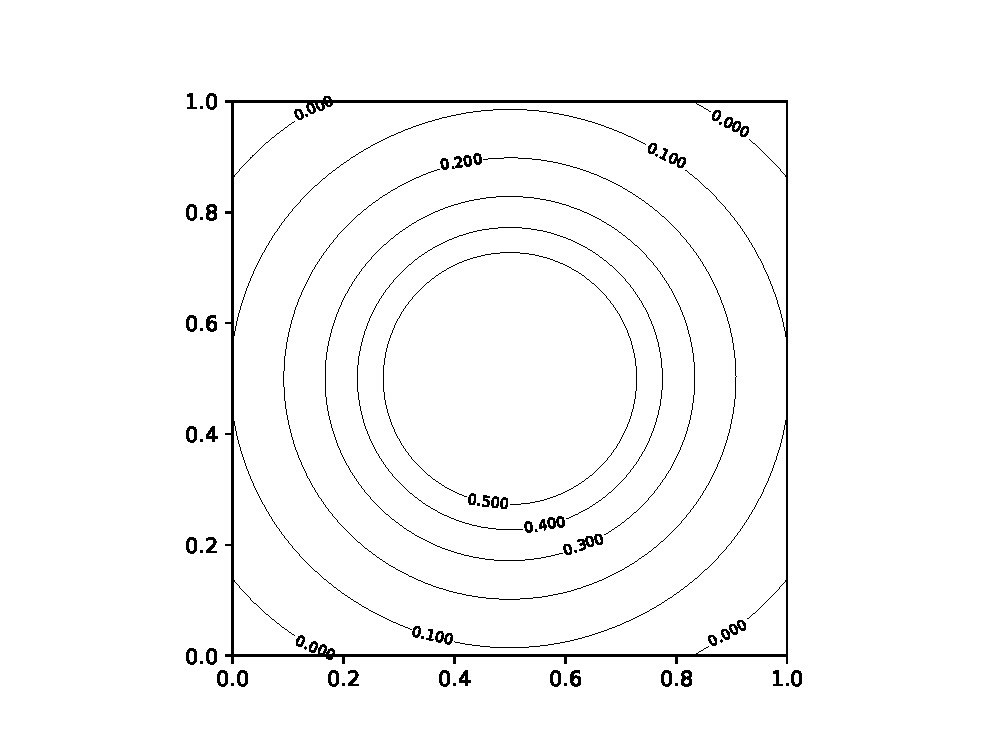
\includegraphics[width=1\linewidth]{jvm-2022/2_phi}
        \\ б) $\varphi$
    \end{minipage}
    \caption{Результаты второго эксперимента}
    \label{fig:4_4:6}
\end{figure}
Рассмотрим двумерный случай: имеется квадрат
$S = \{(x, y), 0 \leq x,y,z \leq 1~\text{см.}\}$ с
круговой полостью $R$ с центром $b_0 =\{0.5, 0.5\}$
$R = \{r, \| r - b_0 \| \leq 0.15~\text{см.} \}$.
Рассматриваемая область $\Omega = S \setminus R$.
$\Gamma \equiv \partial \Omega = \partial C \cup \partial B$ при этом
$ \Gamma_2 = \partial R, \Gamma_1 = \partial S \setminus \Gamma_2$.
Параметры среды возьмём из примера~1.
Граничные данные $q_b$ и $\theta_b$ положим равными
\begin{gather*}
    \theta_b = 0.5, \\
    q_b =
    \begin{cases}
        0.2, & \text{если } x \in \Gamma_1 \\
        -0.2, & \text{если } x \in \Gamma_2.
    \end{cases}
\end{gather*}

Начальное значение функционала качества $0.045$
после тридцати итераций становится равным $6.2\cdot10^{-5}$.
Полученное состояние представлено рисунками ~\ref{fig:4_4:6}а,~\ref{fig:4_4:6}б.


Представленные численные примеры демонстрируют,
что предложенный алгоритм успешно справляется
с нахождением численного решения задачи~\eqref{eq:2_4:eq1}--\eqref{eq:2_4:bc2}
с данными Коши для температуры на части границы.
